\section{Conjunto de datos}

El desarrollo del modelo basado en aprendizaje profundo requiere un conjunto de 
datos apropiado para el entrenamiento.
Para poder realizar el pronóstico de tormentas eléctricas se utilizarán los
datos de densidad de destellos por área (Flash Extent Density, FED), obtenida a
partir del producto GLM-L2-LCFA (Geostationary Lightning Mapper Level 2
Lightning Detection) del satélite GOES-16.

\subsection{Geostationary Lightning Mapper Level 2 Lightning Detection}
El producto de detección de rayos contiene una lista de destellos de rayo, 
acompañado de sus grupos y eventos constituyentes.

\textbf{Evento: }Un evento es definido como la ocurrencia de un solo pixel de
sensor que excede el umbral base durante un periodo de 2ms.
Se debe señalar que un evento puede ser ocasionado por ruido que exceda el
umbral base, en ese caso el evento es una falsa alarma.

\textbf{Grupo: }La descarga de un rayo normalmente ilumina más de un pixel
durante el intervalo de tiempo.
El resultado es dos o más eventos adyacentes durante el mismo periodo de tiempo.
Cuando estos eventos múltiples sean adyacentes (compartan un lado o esquina en
común), serán colocados en el mismo grupo.
La definición formal de un grupo es uno o más eventos simultaneos registrados
en pixeles adyacentes.

\textbf{Destello: }Un destello de rayo es definido como un conjunto de grupos 
secuencialmente separados en el tiempo por 330ms o menos y en espacio por no 
más de 16.5km.
Para que dos grupos sean considerados parte del mismo destello, es necesario
que dos eventos cualquiera de los grupos cumplan la separación de 330ms y
16.5km.
No se utilizan los centroides de los grupos para determinar si dos grupos son
parte de un destello.

\begin{figure}[H]
  \centering
  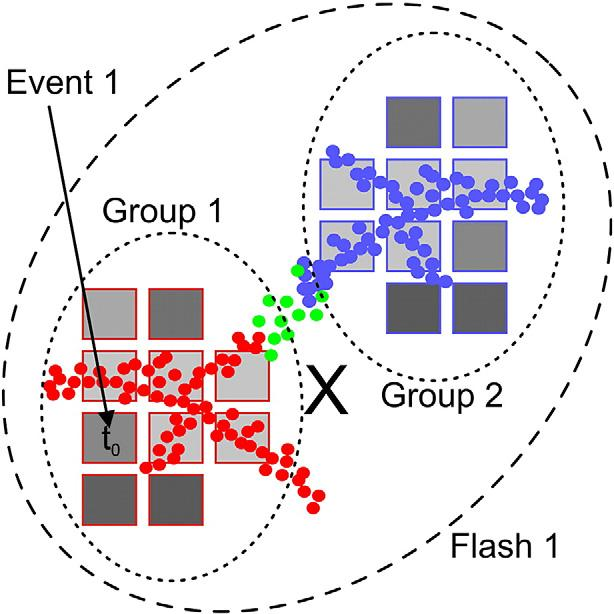
\includegraphics[width=6cm]{E_IMAGENES/5_Metodologia/flash_group_event}
  \caption[Destello del GLM]{
    Ilustración de un destello del GLM compuesto de 2 grupos y 20 eventos.
    \newline
    Fuente:\citep{GOODMAN201334}
  }
  \label{fig:fed}
\end{figure}

\subsubsection{Características de los datos publicados}
Los datos son distribuidos por la National Oceanic and Atmospheric 
Administration (NOAA) en archivos NetCDF-v4 a través de Amazon Web Services
(AWS) o Google Cloud Platform (GCP) con frecuencia de 20 segundos.
Cada archivo contiene:

\textbf{Dimensiones: }
\begin{itemize}
  \item number\_of\_flashes
  \item number\_of\_groups
  \item number\_of\_events
  \item number\_of\_time\_bounds
  \item number\_of\_field\_of\_view\_bounds
  \item number\_of\_wavelength\_bounds
\end{itemize}

\begin{table}[H]
  \centering
  \small
  \label{tab:vars_events_glm}
  \caption{
    Variables de eventos contenidas en un archivo del producto GLM-L2-LCFA del 
    satélite GOES-16
  }
  \begin{tabular}{l|p{3cm}|p{1.15cm}|p{3.5cm}}
    \textbf{Nombre} & 
    \textbf{Nombre largo} & 
    \textbf{Tipo de dato} & 
    \textbf{Atributos} \\ \hline

    event\_id & 
    Identificador único para el producto de eventos de rayo. &
    Int32 &
    {Sin signo}\\ \hline

    event\_time\_offset &
    Tiempo de ocurrencia del evento. &
    Int16 &
    \parbox[t]{3.5cm}{Sin signo \\ Escalado \\ Compensado \\ Medido en segundos desde una fecha}\\ \hline
    
    event\_lat &
    Coordenada de latitud del evento. &
    Int16 &
    \parbox[t]{3.5cm}{Sin signo \\ Escalado \\ Compensado \\ Medido en grados norte}\\ \hline

    event\_lon &
    Coordenada de longitud del evento. &
    Int16 &
    \parbox[t]{3.5cm}{Sin signo \\ Escalado \\ Compensado \\ Medido en grados este}\\ \hline

    event\_energy &
    Energía radiante del evento &
    Int16 &
    \parbox[t]{3.5cm}{Sin signo \\ Escalado \\ Compensado \\ Medido en Joules}\\ \hline

    event\_parent\_group\_id &
    Identificador único para el producto del grupo al que pertenece el evento. &
    Int32 &
    \parbox[t]{3.5cm}{Sin signo}\\
  \end{tabular}
\end{table}

\begin{table}[H]
  \centering
  \small
  \caption{
    Variables de grupos contenidas en un archivo del producto GLM-L2-LCFA del
    satélite GOES-16
  }
  \label{tab:vars_groups_glm}
  \begin{tabular}{l|p{3cm}|p{1.15cm}|p{3.5cm}}
    \textbf{Nombre} & 
    \textbf{Nombre largo} & 
    \textbf{Tipo de dato} & 
    \textbf{Atributos} \\ \hline

    group\_id &
    Identificador único para el producto del grupo.&
    Int32 &
    \parbox[t]{3.5cm}{Sin signo}\\ \hline

    group\_time\_offset &
    Tiempo de ocurrencia promedio de los eventos constituyentes del grupo.&
    Int16 &
    \parbox[t]{3.5cm}{Sin signo \\ Escalado \\ Compensado \\ Medido en segundos desde una fecha}\\ \hline

    group\_frame\_time\_offset &
    Tiempo de ocurrencia promedio de los eventos constituyentes del grupo.&
    Int16 &
    \parbox[t]{3.5cm}{Sin signo \\ Escalado \\ Compensado \\ Medido en segundos desde una fecha}\\ \hline

    group\_lat &
    Centroide del grupo (media ponderada de los eventos por su energía).&
    Float32 &
    \parbox[t]{3.5cm}{Medido en grados norte}\\ \hline

    group\_lon &
    Centroide del grupo (media ponderada de los eventos por su energía).&
    Float32 &
    \parbox[t]{3.5cm}{Medido en grados este}\\ \hline

    group\_area &
    Cobertura de área por grupo (pixeles que contienen al menos un evento constituyente).&
    Int16 &
    \parbox[t]{3.5cm}{Sin signo \\ Acotado \\ Escalado \\ Compensado \\ Medido en m$^2$}\\ \hline

    group\_energy &
    Energía radiante del grupo&
    Int16 &
    \parbox[t]{3.5cm}{Sin signo \\ Acotado \\ Escalado \\ Compensado \\ Medido en Joules}\\ \hline

    group\_parent\_flash\_id &
    Identificador unico para el producto del destello asociado al grupo.&
    Int16 &
    \parbox[t]{3.5cm}{Sin signo}\\ \hline

    group\_quality\_flag &
    Indicador de calidad de los datos del grupo.&
    Int16 &
    \parbox[t]{3.5cm}{Sin signo \\ Acotado}\\ 

  \end{tabular}
\end{table}

\begin{table}[H]
  \centering
  \small
  \caption{
    Variables de destellos contenidas en un archivo del producto GLM-L2-LCFA del
    satélite GOES-16
  }
  \label{tab:vars_flash_glm}
  \begin{tabular}{l|p{3cm}|p{1.15cm}|p{3.5cm}}
    \textbf{Nombre} & 
    \textbf{Nombre largo} & 
    \textbf{Tipo de dato} & 
    \textbf{Atributos} \\ \hline

    group\_id &
    Identificador único para el producto del destello.&
    Int16 &
    \parbox[t]{3.5cm}{Sin signo}\\ \hline

    flash\_time\_offset\_of\_first\_event &
    Tiempo de ocurrencia del primer evento constituyente del destello. &
    Int16 &
    \parbox[t]{3.5cm}{Sin signo \\ Escalado \\ Compensado \\ Medido en segundos desde una fecha}\\ \hline

    flash\_time\_offset\_of\_last\_event &
    Tiempo de ocurrencia del último evento constituyente del destello. &
    Int16 &
    \parbox[t]{3.5cm}{Sin signo \\ Escalado \\ Compensado \\ Medido en segundos desde una fecha}\\ \hline

    flash\_frame\_time\_offset\_of\_first\_event &
    Tiempo de ocurrencia del primer evento constituyente del destello. &
    Int16 &
    \parbox[t]{3.5cm}{Sin signo \\ Escalado \\ Compensado \\ Medido en segundos desde una fecha}\\ \hline

    flash\_frame\_time\_offset\_of\_last\_event &
    Tiempo de ocurrencia del último evento constituyente del destello. &
    Int16 &
    \parbox[t]{3.5cm}{Sin signo \\ Escalado \\ Compensado \\ Medido en segundos desde una fecha}\\ \hline

    flash\_lat &
    Centroide del destello (media ponderada de los eventos por su energía). &
    Float32 &
    \parbox[t]{3.5cm}{Medido en grados norte}\\ \hline

    flash\_lon &
    Centroide del destello (media ponderada de los eventos por su energía). &
    Float32 &
    \parbox[t]{3.5cm}{Medido en grados este}\\ \hline

    flash\_area &
    Cobertura de área por destello (pixeles que contienen al menos un evento constituyente). &
    Int16 &
    \parbox[t]{3.5cm}{Sin signo \\ Acotado \\ Escalado \\ Compensado \\ Medido en m$^2$}\\ \hline

    flash\_energy &
    Energía radiante del destello. &
    Int16 &
    \parbox[t]{3.5cm}{Sin signo \\ Acotado \\ Escalado \\ Compensado \\ Medido en Joules}\\ \hline

    flash\_quality\_flag &
    Indicador de calidad de los datos del destello. &
    Int16 &
    \parbox[t]{3.5cm}{Sin signo \\ Acotado }\\ 

  \end{tabular}
\end{table}

\subsection{Densidad de Destellos por Área}
Para poder utilizar el método de aprendizaje profundo escogido es necesario 
contar con una representación matricial de los datos.
La Densidad de Destellos por Área cuenta el número de destellos detectados en
una unidad de área.
Para obtener la Densidad de Destellos por Área se acumularán los destellos
registrados en los datos crudos del producto GLM-L2-LCFA en grillas.
Esta transformación permite capturar la naturaleza espacial de los datos.

Al realizar el grillado de los datos se obtendrán archivos con las siguientes 
características:

\begin{itemize}
  \item Como mínimo 2 dimensiones de latitud y longitud.
  \item Una variable de densidad de destello cuyas dimensión sea latitud\times
  longitud.
  \item Una variable que indique el tiempo inicial y final de los eventos 
  considerados.
\end{itemize}

Inicialmente se consideró apropiada una grilla de 2km\times 2km debido a que
otros productos del satélite GOES-16 se distribuyen en la misma resolución, y
durante periodos de 5 minutos, para el periodo 2018--2021.
Luego de observar ciertos artefactos en las grillas de 2km\times 2km se decidió
reescalar las observaciones a un múltiplo de la resolución original, siendo la
escala escogida 8km\times 8km.

Los datos (resolución original y reescalada) fueron alojados por el usuario
tesista3 en el servidor de SENAMHI (190.119.131.51).

\begin{figure}[H]
  \centering
  \begin{subfigure}{0.4\textwidth}
    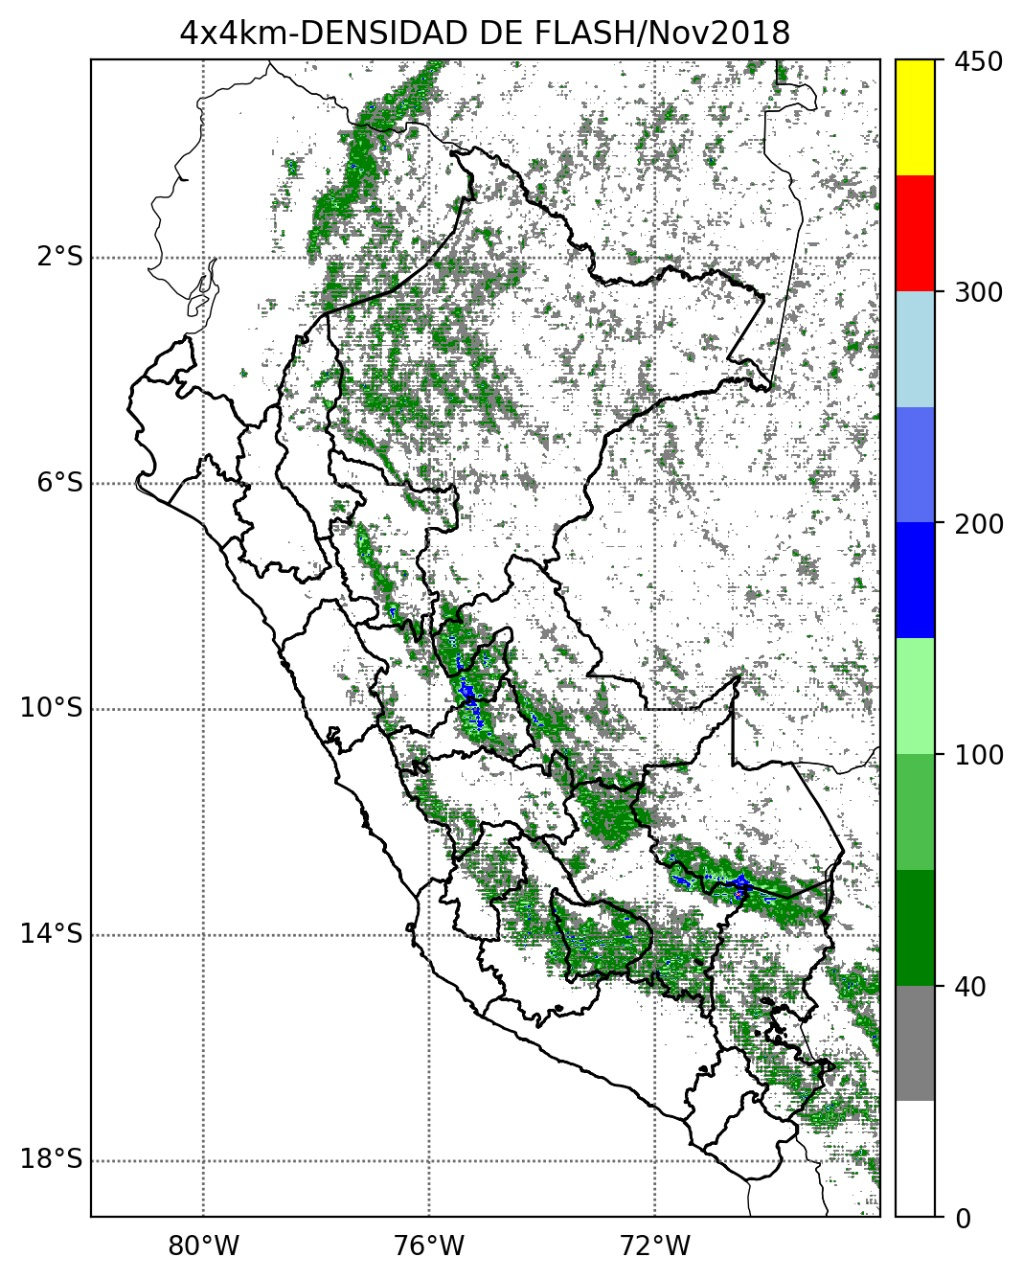
\includegraphics[height=8cm]{E_IMAGENES/5_Metodologia/fed_4_4}
    \caption{4km\times 4km}
  \end{subfigure}\hfil
  \begin{subfigure}{0.4\textwidth}
    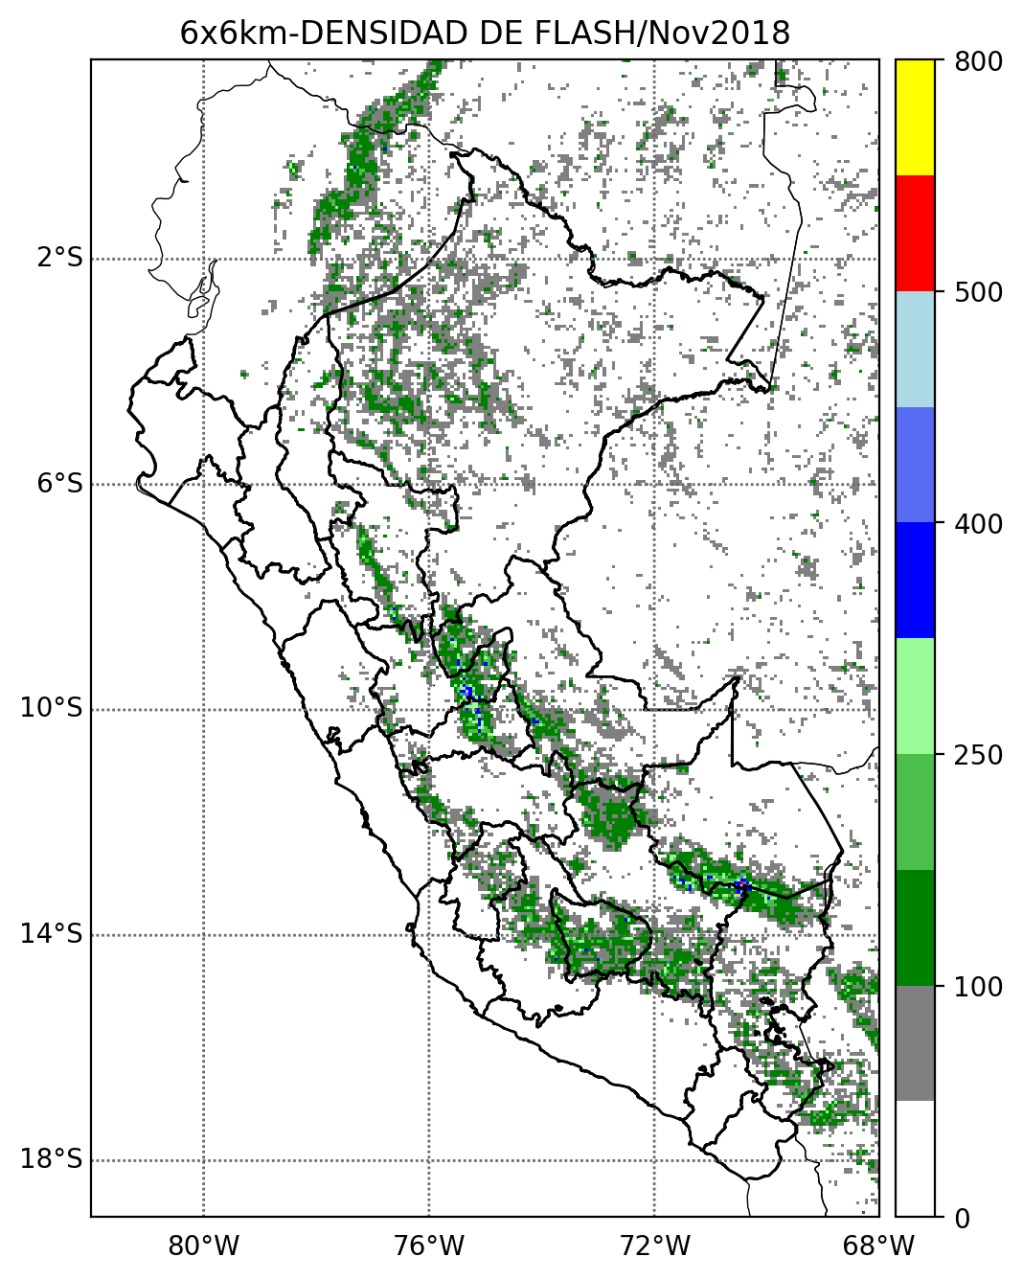
\includegraphics[height=8cm]{E_IMAGENES/5_Metodologia/fed_6_6}
    \caption{6km\times 6km}
  \end{subfigure}
  \medskip
  \begin{subfigure}{0.4\textwidth}
    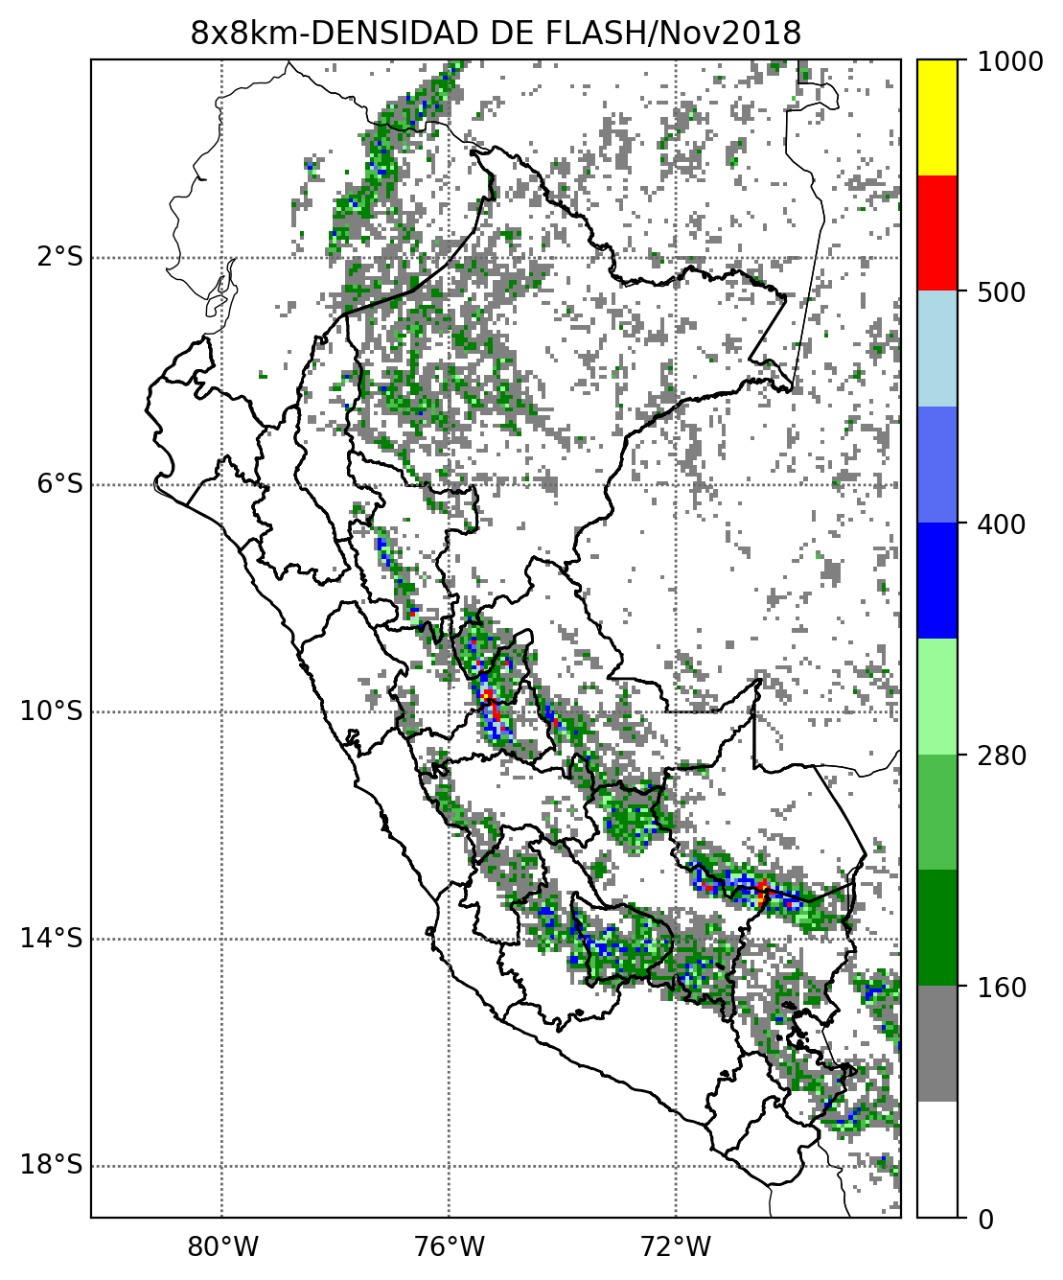
\includegraphics[height=8cm]{E_IMAGENES/5_Metodologia/fed_8_8}
    \caption{8km\times 8km}
  \end{subfigure}\hfil
  \begin{subfigure}{0.4\textwidth}
    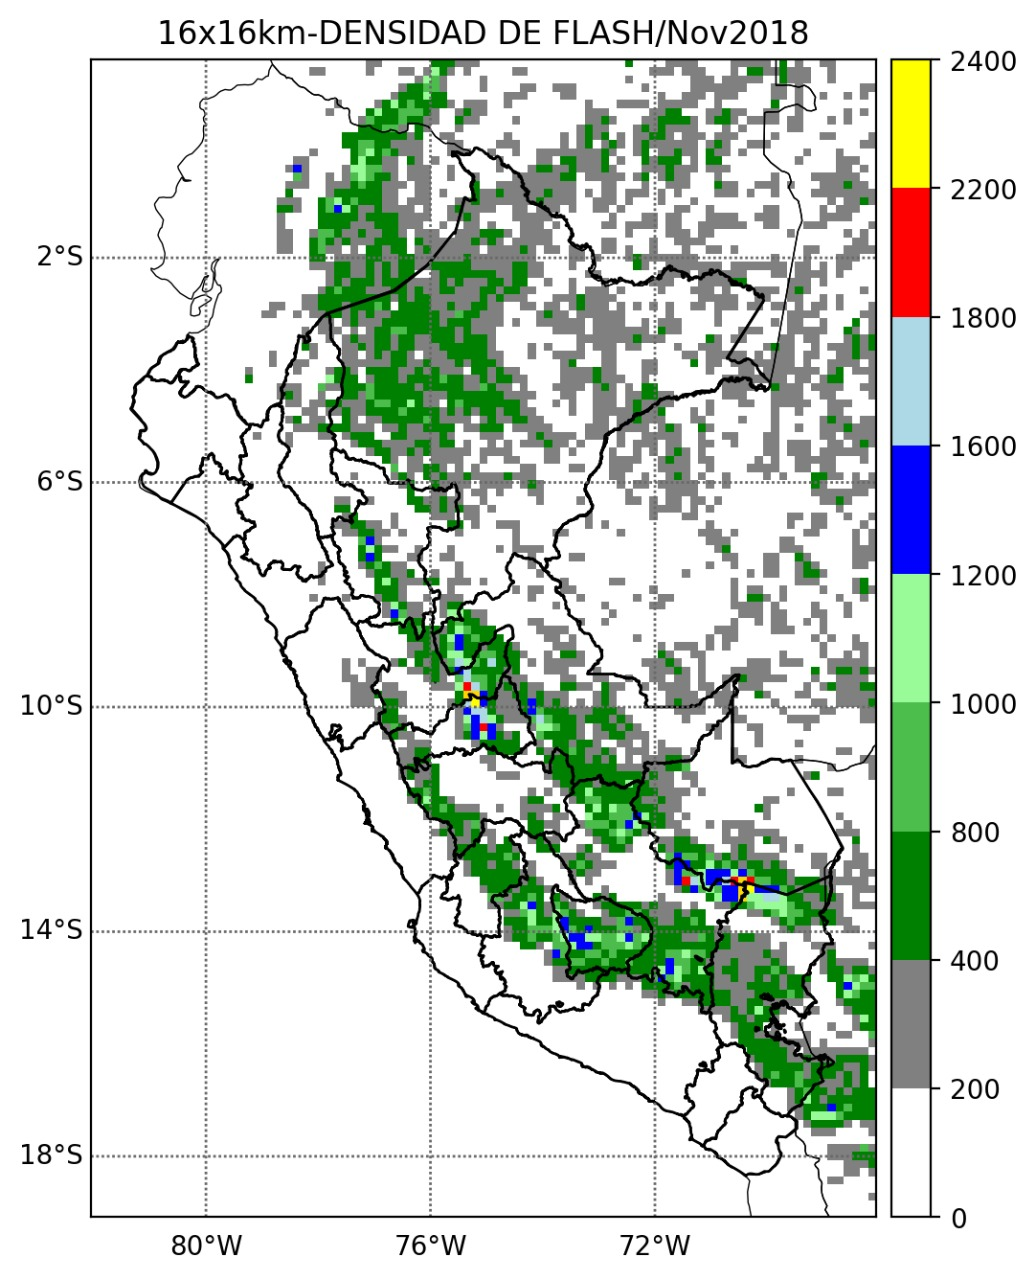
\includegraphics[height=8cm]{E_IMAGENES/5_Metodologia/fed_16_16}
    \caption{16km\times 16km}
  \end{subfigure}
  \caption[Densidad de Destellos por Área]{
    Densidad de Destellos por Área a diferentes resoluciones espaciales.
  }
  \label{fig:feds}
\end{figure}